\documentclass{article}
\usepackage{circuitikz}
\usepackage[margin=1in]{geometry}
\usepackage{xcolor}

% Color Definitions
\definecolor{txtbkwhite}{RGB}{255,255,255}
\definecolor{txtbkprimary}{RGB}{255,51,51}
\definecolor{txtbkpaleprimary}{RGB}{255,153,153}

\usetikzlibrary{calc}

\def\setupMultiplexerDown#1#2#3{
  \coordinate (Mux #1) at (#2,#3);
  \coordinate (Mux #1 O1) at (#2 - 0.5,#3 + 0.25);
  \coordinate (Mux #1 O2) at (#2,#3 + 0.25);
  \coordinate (Mux #1 O3) at (#2 + 0.5,#3 + 0.25);
  \coordinate (Mux #1 I1) at (#2,#3 - 0.25);
  \coordinate (Mux #1 O41) at (#2 - 0.6, #3 + 0.25);
  \coordinate (Mux #1 O42) at (#2 - 0.2, #3 + 0.25);
  \coordinate (Mux #1 O43) at (#2 + 0.2, #3 + 0.25);
  \coordinate (Mux #1 O44) at (#2 + 0.6, #3 + 0.25);
  \coordinate (Mux #1 M) at (#2 + 0.75,#3);
}

\def\drawMultiplexerDown#1{
  \draw (#1) node[anchor=center] {
    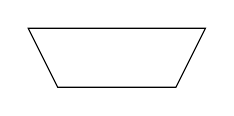
\begin{tikzpicture}[rotate=-90,scale=1.5]
      \draw[fill=white] (0,0) -- (0,1.5) -- (0.5,1.25) -- (0.5,0.25) -- cycle;
    \end{tikzpicture}
  }
}

\def\drawDoubleBentWire#1#2{
  \draw (#1) |- ($0.5*($(#1) + (#2)$)$) -| (#2)
}

\begin{document}
\section{Fetch Stage Diagram}
\begin{tikzpicture}
  \draw (0,0) node[rotate=0] {
    \begin{circuitikz}
      \def\maxBar{4}
      \def\minBar{-15}

      \coordinate (i wb read data) at (1,\maxBar);
      \coordinate (i iaddress) at (4,\maxBar);
      \coordinate (i conflict) at (-3,\maxBar);
      \coordinate (i exec stall) at (-6,\maxBar);
      \coordinate (i mem stall) at (-9,\maxBar);
      \coordinate (o fetch instruction) at (-2,\minBar);
      \coordinate (o fetch stall) at (-8,\minBar);
      \coordinate (o wb req) at (-5.5,\minBar);
      \coordinate (uncached instruction read) at (1,-2);
      \coordinate (sel cache) at (0,-4);
      \coordinate (0xFFEEDDCC) at (-2,-1);
      \coordinate (I Cache) at (-6,0);
      \coordinate (I Cache crd) at (-5,0);
      \coordinate (I Cache ucir) at (-6,-1);
      \coordinate (I Cache icwbreq) at (-7,-1);
      \coordinate (cache read data) at (-5.05,-1.45);
      \coordinate (wb thingy) at (-6.75,-6.35);

      \setupMultiplexerDown{Addr}{0}{0}
      \setupMultiplexerDown{NoCache}{-1}{-2}
      \setupMultiplexerDown{SelCache}{-2}{-4}

      % Gates
      \draw (-6.5,-4) node[or port,rotate=-90] (or1) {};
      \draw (-6.78,-5.95) node[and port,rotate=-90] (and1) {};
      \draw (-6.5,-8.5) node[or port,rotate=-90] (or2) {};
      \draw (-7,-10.25) node[and port,rotate=-90] (and2) {};
      \draw (-8,-12) node[or port,rotate=-90] (or3) {};
      \draw (-6,1.5) node[or port,rotate=-90] (or4) {};

      % Wire Connections
      \drawDoubleBentWire{Mux Addr I1}{Mux NoCache O3};
      \drawDoubleBentWire{Mux NoCache I1}{Mux SelCache O3};
      \drawDoubleBentWire{i wb read data}{Mux Addr O2};
      \draw (i iaddress) |- (Mux Addr M);
      \draw (uncached instruction read) -- (Mux NoCache M);
      \draw (sel cache) -- (Mux SelCache M);
      \draw (o fetch instruction) -- (Mux SelCache I1);
      \drawDoubleBentWire{0xFFEEDDCC}{Mux NoCache O1};
      \drawDoubleBentWire{I Cache crd}{Mux SelCache O1};
      \drawDoubleBentWire{or1.in 1}{I Cache ucir};
      \drawDoubleBentWire{or1.in 2}{I Cache icwbreq};
      \drawDoubleBentWire{or1.out}{-5.5,-4.55};
      \draw (or1.out) -- (and1.in 1);
      \drawDoubleBentWire{-5.5,-4.55}{o wb req};
      \draw (and1.out) -- (or2.in 2);
      \draw let \p1 = (or2.in 1) in
            let \p2 = (o wb req) in
            (\x1,\y1) -- (\x2,\y1);
      \drawDoubleBentWire{or2.out}{and2.in 1};
      \drawDoubleBentWire{and2.out}{or3.in 1};
      \draw (or4.out) -- (I Cache);
      \draw (i exec stall) -- (-6,2.4);
      \drawDoubleBentWire{i mem stall}{or4.in 2};
      \drawDoubleBentWire{i conflict}{or4.in 1};
      \drawDoubleBentWire{or3.out}{o fetch stall};
      \draw () -- () -- () -- ();

      \draw[fill=white] let \p1 = (and1.in 2) in
        (\x1,\y1-1mm) circle (1mm);

      \draw[fill=white] let \p1 = (and2.in 2) in
        (\x1,\y1-1mm) circle (1mm);

      % Multiplexers
      \drawMultiplexerDown{Mux Addr};
      \drawMultiplexerDown{Mux NoCache};
      \drawMultiplexerDown{Mux SelCache};

      % Instruction Cache
      \draw (I Cache) node[anchor=center] {
        \begin{tikzpicture}
          \draw[fill=txtbkpaleprimary] (0,0) rectangle (3,2);
          \draw (1.5,1) node[anchor=center] {\texttt{I\_Cache}};
        \end{tikzpicture}
      };

      % I don't know what this is
      \draw (wb thingy) node[anchor=center] {
        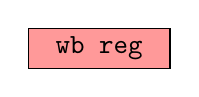
\begin{tikzpicture}
          \draw[fill=txtbkpaleprimary] (0,0) rectangle (1.8,0.5);
          \draw (0.9,0.25) node[anchor=center] {\texttt{wb reg}};
        \end{tikzpicture}
      };

      % Labels
      \draw (i wb read data) node[anchor=south] {
        \begin{tabular}{c}
          \texttt{i\_wb\_read\_data}\\
          \texttt{[127:96] [95:64]}\\
          \texttt{[63:32] [31:0]}\\
        \end{tabular}
      };
      \draw (i iaddress) node[anchor=south] {\texttt{i\_iaddress}};
      \draw (uncached instruction read) node[anchor=west] {\texttt{uncached\_instruction\_read}};
      \draw (sel cache) node[anchor=west] {\texttt{sel\_cache}};
      \draw (o fetch instruction) node[anchor=north] {\texttt{o\_fetch\_instruction}};
      \draw (0xFFEEDDCC) node[anchor=south] {\texttt{0xFFEEDDCC}};
      \draw (cache read data) node[anchor = north west] {\texttt{cache\_read\_data}};
      \draw (o fetch stall) node[anchor=north] {\texttt{o\_fetch\_stall}};
      \draw (o wb req) node[anchor=north] {\texttt{o\_wb\_req}};
      \draw (i mem stall) node[anchor=south] {\texttt{i\_mem\_stall}};
      \draw (i exec stall) node[anchor=south] {\texttt{i\_exec\_stall}};
      \draw (i conflict) node[anchor=south] {\texttt{i\_conflict}};
    \end{circuitikz}
  };
\end{tikzpicture}
\end{document}